%==============================================
\subsection{Gap Ranking Strategy}
\label{subsec:gap}
When no clearance-$W$ path exists, we rank \emph{blocking gaps} on the reachable frontier and expand the most promising one first. The score is obtained by a short A$^\ast$-style \emph{presearch} that predicts the end-to-end \emph{cost-to-connect} if we cross a candidate gap now and then continue across subsequent frontiers.
%------------------------------
\begin{algorithm}[t]
\small
\caption{Frontier Presearch for Gap Ranking (compact)}
\label{alg:gap-ranking}
\DontPrintSemicolon
\SetKwInOut{Input}{In}\SetKwInOut{Output}{Out}
\Input{$\mathbf{s}^{\texttt{S}}$, $\mathbf{s}^{\texttt{G}}$, WCCG, $\lambda_{\mathrm{trans}}$, $\lambda_{\mathrm{push}}$}
\Output{First-hop gaps ranked by predicted cost}
$(\mathcal{L},\texttt{conn})\!\leftarrow\!\texttt{BugFrontier}(\mathbf{s}^{\texttt{S}},\mathbf{s}^{\texttt{G}})$;\;
\If{\texttt{conn}}{\Return $\emptyset$}
$\mathcal{C}\!\leftarrow$ bridge–bridge gaps on $\mathcal{L}$;\;
\For{$g\in\mathcal{C}$}{
  $J_1\!\leftarrow\!\lambda_{\mathrm{trans}}\mathsf{C}_{\mathrm{trans}}+\lambda_{\mathrm{push}}\kappa(g)[\max(0,W-w(g))+\delta]$;\;
  $(\texttt{succ},J_{\mathrm{tail}})\!\leftarrow\!\texttt{PresearchAfter}(g)$;\;
  $\widehat{\mathrm{Cost}}(g)\!\leftarrow\!J_1+\big(\texttt{succ}?J_{\mathrm{tail}}:\infty\big)$;\;
}
\Return $\mathrm{argsort}_{g\in\mathcal{C}}\widehat{\mathrm{Cost}}(g)$ (asc.)\;
\end{algorithm}


\begin{figure}[t]
  \centering
  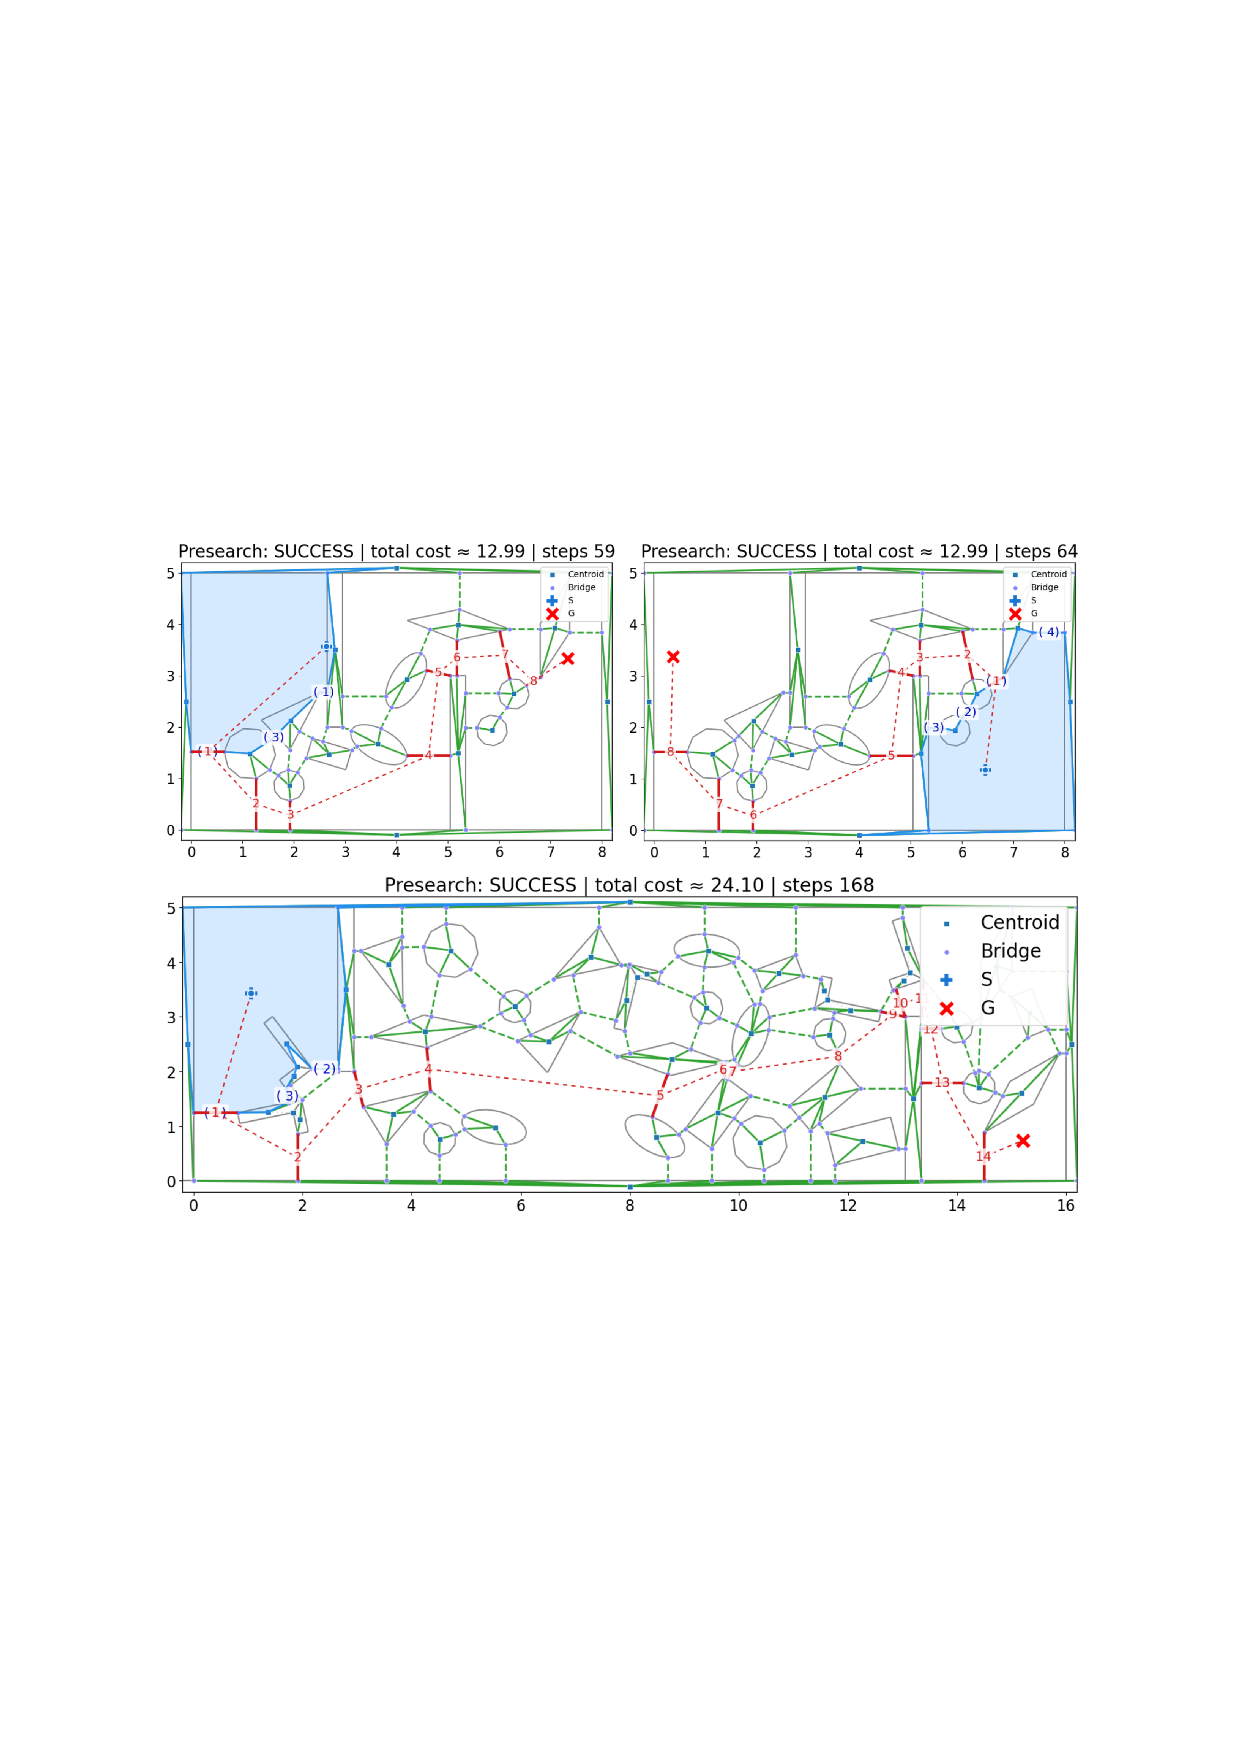
\includegraphics[width=\linewidth]{figures/presearch.pdf}% or {presearch.pdf}
  \vspace{-2mm}
  \caption{
  \textbf{Frontier presearch and gap prioritization.}
  Each panel overlays the WCCG together with the currently selected face (light blue). 
  Numbers in \textbf{red} mark the \emph{gap-crossing order} returned by the presearch, 
  and numbers in \textbf{blue} indicate the \emph{local ranking} of first-hop gaps on the current face boundary.
  \textbf{Top left/right:} the same scene with start/goal swapped, results in symmetric gap orders with same cost (\(\approx 12.99\)).
  \textbf{Bottom:} a longer map with \(\sim 30\) obstacles, showing a 14-gap sequence with cost \(\approx 40.36\).
  }
  \label{fig:presearch}
  \vspace{-3mm}
\end{figure}
%------------------------------
%------------------------------
\subsubsection{Frontier and candidates.}
Given $(\mathbf{s}^{\texttt{S}},\mathbf{s}^{\texttt{G}})$, 
a bug-style query on the WCCG either certifies connectivity or 
returns a counter-clockwise \emph{frontier loop} $\mathcal{L}$ 
that separates start and goal (Sec.~\ref{subsubsec:bugplanner}). 
The \emph{first-hop} candidate set $\mathcal{G}(\mathcal{L})=\{g_1,\dots,g_K\}$ 
consists of visible bridge–bridge edges on~$\mathcal{L}$.

%------------------------------
\subsubsection{Step cost.}
For a gap $g\in\mathcal{G}(\mathcal{L})$, we define the one-hop cost
\begin{equation}\label{eq:step-cost}
J(g\,|\,\mathcal{L},\mathbf{s}) \;=\;
\lambda_{\mathrm{trans}}\,\mathsf{C}_{\mathrm{trans}}(\mathbf{s}\!\to\! g)
\;+\;
\lambda_{\mathrm{push}}\,\mathsf{C}_{\mathrm{push}}(g),
\end{equation}
where $\mathsf{C}_{\mathrm{trans}}$ is the straight-line approach from the current robot center $\mathbf{s}$ to the outside insertion point of $g$ on~$\mathcal{L}$, and the widening term
\begin{equation}\label{eq:push-cost}
\mathsf{C}_{\mathrm{push}}(g)
\;=\;
\kappa(g)\,\Big(\max\{0,\,W-w(g)\}+\delta\Big)
\end{equation}
scales the geometric shortfall $W-w(g)$ by a mass factor $\kappa(g)=\phi(\min\{M_u,M_v\})\ge 1$ of the lighter adjacent obstacles $(u,v)$; a simple choice is
$\phi(m)=1+\alpha/(m+\varepsilon)$ (heavier sliders $\Rightarrow$ larger cost). We add a small margin $\delta>0$ for robustness.  
A consistent one-step heuristic is
\begin{equation}\label{eq:gap-heuristic}
h(g) \;=\; \eta \,\big\|\mathbf{o}(g)-\mathbf{s}^{\texttt{G}}\big\|_2,
\end{equation}
with $\mathbf{o}(g)$ the outside point of $g$ and $\eta>0$ a scale; this is an admissible proxy for the remaining crossings and empirically stabilizes the presearch.

%------------------------------
\subsubsection{Presearch ranking.}
For each first-hop $g$, we run a short beam/A$^\ast$ that: (i) \emph{virtually} crosses $g$, (ii) recomputes the next frontier $\mathcal{L}'$, and (iii) enqueues the top-$B$ gaps on $\mathcal{L}'$ by priority $f = g\text{-cost} + J(\cdot) + h(\cdot)$. The process stops when the start and goal become connected (success) or a small depth/queue budget is reached (cut). The predicted end-to-end score of $g$ is
\begin{equation}\label{eq:total-cost}
\widehat{\mathsf{Cost}}(g) \;=\;
J\!\big(g \mid \mathcal{L}, \mathbf{s}^{\texttt{S}}\big)
\;+\!\!\!\sum\nolimits_{g'\in\Pi^*(g)}\!\!\! J\!\big(g' \mid \cdot \big),
\end{equation}
where $\Pi^*(g)$ is the subsequent gap sequence discovered by the presearch after crossing $g$. We rank in ascending $\widehat{\mathsf{Cost}}(g)$.


\subsubsection{Efficiency notes.}
We cache frontier loops and memoize $(\mathcal{L},g)\!\mapsto\!\mathcal{L}'$ transitions; 
nearest-edge hits are vectorized with AABB culling, 
giving near-linear time per ray-shoot in the number of visible edges. 
The presearch depth/beam $B$ is small (e.g., $6$–$10$), 
so ranking is typically subdominant to the physics loop.